\chapter{风暴}

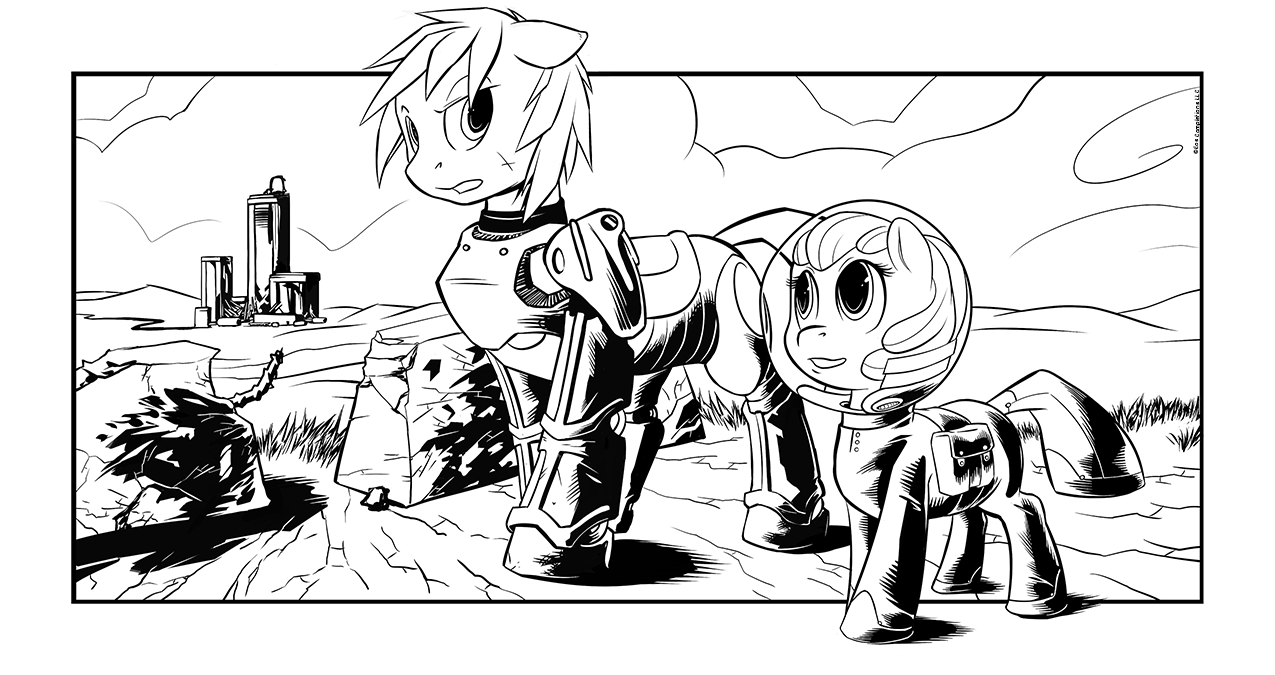
\includegraphics[width=\linewidth]{image13.png}

\begin{intro}
我说,你见过下雨么?
\end{intro}

\daytimeplace{11}{18:00 PM}{象牙塔,52号国道中段}{Ivory Tower, Big 52 SC Branch}

象牙塔是个强化陶瓷外墙的巨大白色建筑。在战前这里曾经是个研究设施,和平部的员工在这里寻找神秘科学部\footnote{神秘科学部 (Ministry of Arcane Science):大战时期由暮光闪闪成立的部门,负责魔法研究,\emph{FoE} 中的天角兽「女神」便是该部门的「产品」之一}和战时科技部\footnote{战时科技部 (Ministry of Wartime Technologies):大战时期由苹果杰克成立的部门,主要通过陆马(物理)方式研发和制造科技产品并用于战争}研究成果的非军事用途。

现在象牙塔是铁骑卫在52号国道的唯一据点,主要因为这里是附近唯一没有被旭日公司碰过的高科技设施,而稍微有些理智的小马都不会碰旭日公司。

没错,旭日公司,那些疯子,他们将一个收音机和一个吸尘器组装在一起做成了第一个声波武器然后交给一个稀里糊涂的女仆。还发明了第一个带有窃贼监测消灭功能的门铃——这个门铃电死了六十多个上门服务小马和一整排的卖马芬小孩子。

整个建筑都被一道带有护城河的城墙围着,并且带有自动炮台和地雷阵。这个城墙经过一个世纪对抗从土匪到山贼的战斗之后。现在看起来相当糟糕。炮台早已经被摧毁,地雷阵也基本没有了,就连城墙也饱经创伤。在唯一还算完好的护城河之上有两座吊桥,一座在西边一坐在北边,在吊桥外面有各式各样的棚屋,大多都是一些旅行商队的仓库以及那些和铁骑卫做生意的小马过夜歇脚的地方。

不过现在北边的棚屋已经基本被拆光了,而各种垃圾被收集起来在桥北边堆出一个路障,同时西边的那些战前建筑也被垒上了沙包,并且飘扬着苹果杰克卫士的旗帜。

这个小小的要塞被一打小马守卫着,其中甚至还有一些穿着战斗鞍的年轻小马。一对武装到牙齿的铁骑卫穿着它们传统的动力装甲正守在桥头。另外一个则带着新兵在象牙塔周围的乱石滩巡逻。第四位则站在临时指挥所里面和一个年轻的佣兵争执着。

「你说的我能做到,但是我现在想先要一半定金,还有一些等离子武器。」赫瑞塔抱着双臂坐在椅子上,把自己的狮子腿翘在桌子上。

那个骑士一脸不爽地摇了摇头:「你当我是啥?卖房车的?我给你一柄动力长矛已经算你好运了,其它的东西只有你完成工作才给你。」

赫瑞塔轻蔑的哼着,「我是个枪手,你那花哨的肉搏兵器我用不上……给我三个离子手雷,现在给我两个,回头再给我一个,还有俩EMP地雷我就依你。」

「给你俩EMP手雷,事成之后再给你一个离子手雷和离子地雷,最终价。」小马用蹄子指着狮鹫说。

赫瑞塔耸了耸肩,抓住那只蹄子握了握,「成交,先付一半瓶盖。」

「然后你拿着钱飞走?我才不信你,而且你现在拿着钱又啥也做不了。」

狮鹫叹了口气:「你知道我怎么想的吗,我觉得你没有那么多瓶盖,你是想让我去捣乱,然后你们正面进攻,最后你们用基地里面的钱付给我……我不觉得你们四个铁骑卫和十五个新兵能够正面攻破一个至少一打半重装备小马防守的城堡。」

那个帕拉丁举起了蹄子,「好吧好吧,你这个守财奴,现在就给你一半瓶盖!别觉得我会因为这件事情感谢你。」

「谢意买不来子弹,我想这可以成交了,」狮鹫又耸了耸肩,「我马上就出发,希望你的手下别把事情搞砸了。」

「你干完活回来和书记梅隆说,如果你想参加正面进攻的话,我会再给你点别的,比如一些收集到的装备。」

赫瑞塔还没开口,但是她面前的小马举起一只蹄子示意她等等。

「冷浴收到,请报告。」小马压低声音,但是狮鹫竖起耳朵也能听得很清楚。

赫瑞塔坐在桌子面前打着哈切,不管怎么这事情和她无关,等到入夜他就出发,想想他们已经允许她从铁骑卫尸体上扒装备了,说明这些小马已经没什么选择了。

「再说一遍?你射杀他多少次了?」那个帕拉丁惊讶的叫起来:「高斯我觉得你不可能杀死一个东西两次以上……」

听到这句话赫瑞转头看着那个用对讲机说话的小马,不过现在冷浴完全没有注意那个佣兵。「你到底想要说什么,你确定那是敌军么?」帕拉丁停顿了一下听着对面的回答然后说:「所以,你只是因为觉得他有点诡异所以就开枪了?」

狮鹫听到这句话跳了起来:「肏你娘,告诉你的手下不准欺负帕比!」

\horizonline

\daytimeplace{11}{18:30 PM}{象牙塔,52号国道中段}{Ivory Tower, Big 52 SC Branch}

黄色的小雌驹,蹦蹦跳跳地来到小小的前线,看着那锈迹斑驳的路障,对上面的卫兵说:「嗨漂漂马!我叫快乐帕比,你看到我妈妈了么?」

内心和身上铠甲一样上锈的卫兵疲惫地看着帕比——他已经被连续几天无休止的战斗折磨得痛苦不堪,而且和他战斗的并不是强盗或者奴隶贩子,而是他曾经的挚友和老师。而这个小雌驹却一点都没在意对方的情绪。

帕比继续和护送她的卫兵讲着自己的故事:「……所以,即使镇长要赶走了机械战马,他还是决定去拯救城市。因为……你懂的,机械战马并不只是个机械,他也是超级厉害有正义感的小马!」小雌驹完全没有注意到那个卫兵不断上升的不耐烦情绪,「但是我刚看到那里妈妈就关了电视不让我看了,我不知道为啥她不允许我看那种电影,你说,机械战马绝对是个好马,所以最后她一定会赢,是吗是吗?」

帕拉丁高斯重重叹了口气:「对,你说的没错,不过我并不是你说的啥机械战马,我是阿杰铁卫!完全不是一回事!」

帕比咯咯笑起来,「你真有趣,机械战马阿杰铁卫!我喜欢这个名字!」

「好吧,……随你便,摆脱,至少把那个肉食灵尸体放起来,恶心死了!」小雌驹还背着那个死去的肉食灵,没有一位小马会对这个已经没有一只腿和一只翅膀的前肉食灵感觉到一丝的怜悯之情,不过小雌驹还是把它当宝贝一样带着。

帕比皱起眉头,「但是小毛球肯定也想看漂漂马,他会乖乖坐好的,我发誓!」

帕拉丁以蹄覆面,「尸体当然会乖乖坐好,但是……哎……恩……这附近有专吃宠物的怪物,所以可能会……」帕拉丁心中默默地对这个幼驹扯谎而自责。

「吃宠物?在哪儿?毛球很危险!」小孩子马上把那个小肉食灵塞进背包里面,睁大眼睛看着周围。「在包包里面躲好,我来收拾他们!」

高斯看着刚好撞上的仨随从笑得满地打滚,哑口无言。而帕比也一起笑起来,「什么事这么有趣?」

高斯避开他们的视线,拿出自己最正经的表情,「这才对,你要小心哦,吃宠物的怪物哪里都有!现在跟我去见长官吧。还有你们仨!别在那里傻笑了,赶紧给我看大门去!」帕拉丁走过那几个年轻随从,小黄驹屁颠屁颠地跟在后面。

「好的好的,阿杰铁卫机械战马!我们什么时候去打击罪犯?」

「我再说最后一次,我的名字叫高斯,帕拉丁高斯!」公马叹息着,「我绝对不会要孩子……」

这对活宝终于走到了指挥部,公马打开门让帕比先走了进来,这个建筑曾经是一个学校,不过现在大部分都已经坍塌,只剩下几个房间还勉强保持完好,在这个小小办公室的另一边坐在桌子后面的是另一个穿着铁甲的小马还有赫瑞塔。

「赫瑞!」帕比开心地一蹦三尺高,径直飞扑向狮鹫,而后者侧身闪开,然后抓住帕比的后颈将她拎了起来。帕比微微挣扎了一下,来回张望着寻找着她的朋友。「嘿,你跑哪去了?」

「我说了『再见』就是改天再见面的意思,你还在往南走么?」狮鹫一边说着一边把帕比放下,拍了拍她的头盔。「帕拉丁伙计,这个是我的老朋友,在我干活的时候能帮我看好她么?」

冷浴歪着头一脸疑惑地看着小雌驹,「这个……小马被射中四次但是看起来毫发无伤的样子,而且她看起来心情不错,我不太清楚我能不能照顾……高斯,叫诘责书记进来。」

帕比并不太关心那个帕拉丁,因为见到赫瑞实在太开心了,「没错哦,妈妈就在桥对面的那个白屋子里面!我路上看到好多漂漂马,还有阿杰铁卫机械战马!」小雌驹终于抱上了狮鹫,「我好高兴见到你,这一次你不会丢下我了吧!」

赫瑞塔清了清喉咙,避开幼驹的视线。「呃,实际上……我正要去做一些事情,不过如果你等我的话,我很快就回来。」

帕比皱了皱眉头,小心地问道:「呃……你会带上丝尾一起去么?」

「丝啥?哦,那个玩偶,当然,为啥不带他?」

小雌驹松了口气,「没什么,让它帮你吧,她很厉害!」

狮鹫拍着小孩子的头说:「很好,乖乖和铁骑卫呆着,别惹他们生气也别乱跑,我一会儿就回来带你玩,好么?」

「耶!」帕比挥着蹄子送走赫瑞,然后呆在房间里面好奇地看着其他马。

\horizonline

\daytimeplace{11}{19:00 PM}{象牙塔,52号国道中段}{Ivory Tower, Big 52 SC Branch}

诘责书记是一个常年负责训练随从的老马,他冷酷而又铁血的训练手段让每一个新兵都对他心有余悸。只有一种办法能让这个老书记看得起你,把每一个任务都完成得尽善尽美。而当他加入阿杰铁卫的时候,很多人都怀疑他的这个选择,甚至很多随从都觉得他是个间谍。

诘责一边看着帕比一边对冷浴说:「中心城尸鬼有和通常尸鬼一样的腐烂外表,我不觉得她像是其中之一。」

帕拉丁叹了口气坐在他办公桌背后,「那你觉得她是什么?她可是挨了四枪,一枪在头上,三枪心脏。」

「也能给我一个红披风么?」帕比抓着诘责的斗篷一脸惊讶地说:「我喜欢金色的东西,就像漂漂大公主的颜色那样!我长大以后我也要做一个公主!我想要这个披风,拜托!」

「这些是咒符,不是给你玩的。乖乖坐好……」诘责回头继续说。「或许是某种死灵巫术,我可以确定……如果我能去图书馆的话我可以做一些研究,不过现在我只能推测……」

「为什么我不能玩儿?我可以给你东西换斗篷!这叫做交易!超酷的!大家都这么做!不像那次我用早餐换了两块大理石然后饿得发慌被妈妈骂……这次没问题的!」

帕拉丁无视帕比,点了点头说。「那么你的推测是什么?」

诘责看了看那个幼驹然后回答:「我不想拿我的斗篷和你换什么,乖乖坐那儿让成年马说话好么?」书记官叹了口气然后继续和冷浴之前的谈话,「我记得读过这些防辐射服的故事,它们显然没什么作用,在中心城的核爆之后几乎每个穿着它的小孩子都变成尸鬼了。」诘责停下来低头看着那个不停地扯着他斗篷的小雌驹,「不过这一个,我要说……或许我给他的防护服做一次检查就知道结果了。」

老书记把他的哔哔小马接上帕比衣服的数据接口,另一个蹄子按着幼驹让她别动,「安静几分钟好么?」

「我能抱抱你么?你好有趣,我喜欢你!」帕比想了想又说。「我也喜欢你的披风,刚才我说过了么?」

冷浴忍不住笑了出来,书记官瞪了她一眼,「好吧,你想怎么抱我就怎么抱我,恩……我们看看结果……」

诘责皱起了眉头,「从数据上看她已经死了,没有心跳,没有体温,甚至都没有身体,只是……两千多个骨头碎片和一百八十克有机物,完全不是尸妖。」

「呦呵,红斗篷也会说不明觉厉的话!」

「没错,诘责,别说那些不明觉厉的话,给我一个士兵听得懂的说法,我只懂轻武器和战车。」冷浴并不是不高兴,只是想提醒一下老书记官他现在并不是在讲课。

「我也不清楚,只能说她不是尸鬼。」诘责低头看着哔哔小马上的分析结果,「这个防护服的自律智能完全没有受损,所以我可以肯定这不是一个疯狂机器……哦,这一条很有趣,主医疗芯片在两百年前就故障了,这可是千分之一的故障率,或许是因为在启动中受到了电流冲击或者短路,所以只有备用护符在起作用。

「这一条哪里有趣了?」冷浴不解。

书记冷笑一声,「因为备用医疗护符和主医疗护符有很大不同。」

帕拉丁打了一个响鼻,「请一次说完好么,我可没时间做课后复习了。」

书记叹了口气,忽略帕拉丁的态度,「这个护符并没有内置医疗法术,只是有一个自动注射医疗药水的功能……等等,这个魔法回路上还刻着其它东西,是……斑马的咒文?医疗护符上刻着斑马咒文有什么用?」

这个咒文的结果现在就站在他们鼻子下面,用力扯着诘责的斗篷,「好吧,那咒语,保存了……一百八十克有机物?」

书记官继续看着他的哔哔小马,「对,这是一个有点腐烂的心脏,我要说……这个非常有趣,扫描表示有很多破碎的子弹漂浮在心脏附近,就好像它们没有命中心脏一样,我们看看护符的日志,或许能理解它的工作原理。」

他们俩聊天的内容太无聊了,帕比虽然是一个很有耐心的孩子,但是全小马国的耐心都没有那些哇啦哇啦哇啦麻烦,所以那个黄色的小雌驹开始把自己的蹄子伸进书记官口袋里面翻起来。她找到……一支笔,几张纸,一本书,一副眼镜……咔嚓……好吧,现在是一个单片眼镜,还有另一个单片……「咦,这是什么?」

帕比从诘责口袋里面掏出一个梳毛塑料玩具,那是一个白绿色鬃毛的独角兽,脸上带着一个大大的微笑,还有一个竖琴的可爱标记。

「哦哦哦,好可爱!」小雌驹抚摸着玩偶的鬃毛,「梳啊梳,梳啊梳……」

「怎么……喂,还给我!」书记官生气地把那玩偶从帕比蹄子上抢下来,然后塞回自己的口袋去。「玩你自己的玩偶好么,这个可动手办很容易就会弄……」诘责的视线对上了冷浴的目光,然后他才意识到发生了什么,「不不不不不不……咳……这个……玩具……恩恩……是我没收别的新兵的,不是我的别玩坏了!」

帕比一下子兴奋地睁大了眼睛,「不是你的?能给我吗?我会好好爱护她,给她梳毛,一起和她玩,我们会成为最好的朋友,就给她起名字叫糖糖\footnote{糖糖和天琴,同人中默认的一对CP}然后给她染个粉毛。」

诘责听到要给玩偶染毛的话之后立刻炸毛了,「她的名字是『天琴』,而且我不能给你,因为那是我……呃……我的一个学生的,应该仔细分类保管好!」

一个贱贱坏笑出现在帕拉丁的嘴边。

「别对一个玩具那么认真嘛诘责书记,我觉得让这个小雌驹玩一个小女孩的玩具没什么问题。」

冷浴一脸黄鼠狼给鸡拜年的坏笑。

「看吧,看吧,机械战马也说我可以玩,给我嘛,给我嘛!给我嘛!!」幼驹踮着脚去探诘责的口袋,但是这一次老书记官连忙捂住了自己的口袋。

「这个是我的总行了吧!天琴是我的!我不能给你因为我喜欢天琴!你满意了吗!嗯?」按下内心自爆按钮的书记官涨红了脸看着冷浴,「你可以从这个大姐姐房间里面挑一个玩偶,我想她会让你看她的卧室的,我想她没什么好藏的东西,对不对啊,机械战警?」

冷浴咳嗽了一下收起了笑容,「好吧,我带你去找几个漂亮玩具,小家伙,不过先乖乖让书记官做完他的工作。」

在新玩具的保证下,帕比一脸开心的表情乖乖坐在那里让红斗篷小马继续摆弄她的防护服。

诘责叹了口气,看了帕拉丁一眼说:「你能不要露出那副阴阳怪气的笑容好么,我干正事呢……」书记官叹着气。

「我的天……没开玩笑吧,他们居然在医疗护符里面放这种东西?」

冷浴一脸迷茫地看着诘责。「你发现什么了?你的脸色看起来不太好。」

「非常糟糕的事情……和平部的某小马为了不让这些小孩子死而做了非常可怕的事情……她不允许他们死掉。」

「什么叫不允许?」帕拉丁抬起一根眉毛问。

「我是说,这个备份护符的最后咒语是某种死灵术,虽然不清楚具体是什么不过看起来它的功能是把患者的生命灵魂束缚在它的遗骸上。」老书记官叹了口气,「不过,这个并不是太强的法术,我想花点时间研究一下就能解除它。不过这又回到了我们之前的问题上了——我需要图书馆。」

冷浴喃喃自语着:「就算是从爱的角度出发,怎么会有马做出这种……禁止你去死的东西,这个有可能么?」

「既然结果已经站在我们面前,我觉得可能,我不是死灵术专家,但是我可以说这个护符状态并不是很好,它在两百年的时间内都只靠一点点能量维持运转……我不知道怎么解释,这个法术逻辑上根本行不通!一定还有其它拼图碎片没有找到……或许……」

帕拉丁歪着头问:「所以说,基本上这个小鬼是某种幽灵?」

诘责摸着下巴,「我不太清楚,我还是需要再研究一下,不管怎么说我觉得这个护符是关键,没有它这只不过是一件破防辐射服,一堆粉色粘液和一个小雌驹的遗骨……你如果说这就是幽灵的话,我不这么认为,技术上讲这个可怜的小家伙根本不可能站起来,但是现在她却和一个孩子一样活蹦乱跳,不管记忆上还是精神上都完全没有问题。」

老书记官顿了顿,揉了揉自己的眼睛然后继续说:「从日志上看,这个防辐射服已经停止运转两个世纪之久,然后忽然它的魔能电池就充满了远高于它最大能量的魔力。整个防护服都以五倍于它理论效率的水平运转……不管从科学上还是魔法上的逻辑都行不通,或许她是小马灵魂的某种具象化?」诘责一脸沉思的表情放开了帕比的蹄子,「好吧,小家伙,检查完了?」

帕比微笑着抬头看着书记官,「耶,现在我就去找妈妈了,回头我回来拿玩具,拜拜!」

\horizonline

\daytimeplace{11}{19:45 PM}{象牙塔,52号国道中段}{Ivory Tower, Big 52 SC Branch}

帕比用力敲着「我要去找妈妈!放我出去!」小雌驹一边哀求着一边敲着门,但是没有马理她,她被困在这间教室了。

那些讨厌的机械战马把她带到这个房间然后说要给她玩具,然后就把她关在了这里,就像商场的托儿中心一样,她讨厌托儿中心……虽然他们也给了她很多玩具彩笔甚至一个超级炫酷的彩图连环画,但是她现在不是玩这些东西的时间,她应该去找她的……「哇哦!这里画着漂漂蝴蝶!」不对,帕比,你必须抵抗诱惑……你应该……「哇哦,金色蜡笔!真的是金色的哦,我可以用这个笔画塞拉斯蒂娅公主,给她涂上金色就和真的一样了!」

不对!妈妈才是首要任务!帕比是有重要任务在身的小雌驹!她放下那些炫酷的连环画和蜡笔,这些\textbf{腐朽奢靡的花哨玩意儿}才不会让她停下脚步!绝对不会!

「咦?着是真的茶具么?还有茶杯!」

帕比一败涂地。

而五分钟之后帕比已经输得找不到北了。

「天啊,毛球小姐吃了瑞瑞女士的万马奔腾庆典礼服!如果没有金色蜡笔的话整个庆典就完蛋了!不过没有关系,漂漂塞拉斯蒂娅公主带着金色蜡笔登场了!还有云宝黛西!庆典得救了!大家一起喝茶庆祝吧!耶!」

帕比举着肉食灵尸体和其它玩偶,自言自语地着专注于她想象中的场景——那个完全变成茶话会的万马奔腾庆典。

诘责看着窗口里面的情形耸了耸肩,「看起来她不会惹什么麻烦,让两个侍从守着大门以防发生什么意外,我们继续准备今晚的进攻计划吧。」

冷浴浑身不自在地跟在诘责的后面,「她看起来暂时有点乐不思蜀,不过这不是长久之计,我们不可能就这样把她关在这里,过不了多久她就又会吵着要找妈妈了吧。」

老马叹了口气:「我想我可以解除她身上的诅咒,那个咒语很弱,不过我还是需要研究一下斑马魔法,而且还需要几个独角兽配合。」

「那样的话……她会死么?」帕拉丁的声音里面充满担忧。

诘责疲惫地转过头,一副沉重的表情严肃地说:「她已经死了,冷浴,这个小家伙现在需要的是安眠,她本来就不应该存在。」

「但是,她又不在乎……我们至少应该找找看她妈妈是不是还活着,或许她变成了尸鬼……如果她还活着,或许图书馆里面会有一些记录。」

书记官耸了耸肩,「那么又回到了我们之前的话题,夺回我们的基地还有图书馆,所以说,找俩侍从看好她吧,我们现在应该讨论一下如何解决眼下的问题了。」

\horizonline

\daytimeplace{11}{22:00 PM}{象牙塔,52号国道中段}{Ivory Tower, Big 52 SC Branch}

再来点粉色云彩……完成咯!帕比开心地看着她的新创作,谁说不能用粉色画画?把所有东西都画成粉色不就行了吗?她拿起来这幅画把它和其它的画贴在……{}

轰隆!

整个窗户颤抖了一下,外面的光芒透过窗户在地板上照出不详的橙红色方格,让帕比惊讶地站住了。

「烟花?」

轰隆隆!

外面又爆出一团红色的火球,窗户整个炸碎了,玻璃的碎片飞得满屋都是,桌子上和帕比的头盔上都是,不过帕比完全不在意,她探出头去好奇地看着外面发生的事情。

「耶!烟花大会!」幸运的帕比这次赶上了漂亮的烟火!就在桥对面,好多好多小马在跑来跑去玩着烟火,相互丢着各种颜色的光线和烟花,果然那些机械战马知道怎么开个超级大派对!

幼驹走到门口才想起来门被锁上了,不过这阻止不了帕比,她直接从窗户跳了出去。

脚踩在外面的地面上,黄色的幼驹稍微迟疑了一下,把那么多玩具和画丢在那里实在太可惜了,软气那次怎么说的来着?总有一天她需要作出牺牲……如果想要前进就要把某些东西留下。帕比就知道那些丑丑马很厉害,又聪明又厉害,还有乐乐姐姐也是!所以她是个有重任在身的小马,而且她也想去看烟花,所以……再见了!漂漂玩具,再见了!蜡笔!哦,她要先去找妈妈!出发!帕比!

\horizonline

\daytimeplace{11}{22:15 PM}{象牙塔,52号国道中段}{Ivory Tower, Big 52 SC Branch}

象牙塔和大桥桥头之间的整个区域都变成了一个战场,四个阿杰铁卫在用他们的重武器压制着对面阵地,而其他侍从则发起进攻,那些只有轻武器和少量铠甲的新兵用血肉之躯发起冲锋,而当帕比穿过大桥的时候,从帕拉丁高斯身边晃过去的时候他完全没有注意到黄色小雌驹。

「草泥马,她在这里干什么?冷浴!幽灵在战场上!」帕拉丁想追上帕比,但是刚露头就被一阵凶猛的火力压回了掩体,「肏,这尼玛出去就是死路,而且不止一条!第二小队需要掩护!」

帕比看到一个年轻雌驹躺在一个冒烟的弹坑旁边,一滩红色的液体正在那静静安睡的年轻雌驹身体下面慢慢扩大。

「喂,漂漂马,你还好么?」帕比看着那个侍从,她虚弱地睁开眼睛。

「请……救救我……我……我不想死……」士兵的声音虚弱得几乎听不到。

小雌驹轻轻抚摸着侍从的鬃毛。「别害怕,烟火是有点小可怕,但是你是个成年马不应该哭的。」

濒死的小马迷茫地看着她,没有听到幼驹安慰的话,「我……我不想死……」她如此年轻,或许才是第一次参加战斗的新兵。

「好了好了……」帕比坐在小马身边,不停地摸着她的鬃毛。「我陪着你,别害怕,已经没有什么好害怕的了……等烟火结束了我们去买棉花糖,好么?」

帕比第一次看烟花也很害怕,但是妈妈给她买了棉花糖她就不哭了,或许这个小马也一样,给她买个好吃的棉花糖她就不哭了。有几发流弹打在帕比身上,但是她完全没有注意。

「妈妈……抱歉……为什么我要离开家?」侍从低声说着她最后的遗言。

「呃……别担心漂漂小马,如果你离家出走妈妈一定会很高兴在看到你的……或许她会训斥你,但是我保证她会抱抱……」但是那个小马并没有回话。

帕比轻轻戳着她。「呃,你还好么?漂漂小马?呃……声音先生?她还好么?」

「{\mt 分析中,否定。阿杰铁卫侍从状态:已死亡。}」

帕比皱起了眉头,「哦,像是赫瑞的爸爸……」帕比似乎终于意识到发生了什么。「声音先生……这些小马在玩还是在打架?」

「{\mt 这些小马在战斗,不过双方都未将你标记为敌对,只有固定防御系统标记为敌对。}」

似乎是要强调那句话一样,爆炸的弹片飞过,打裂了帕比的头盔。

「{\mt 警告,密封失效,修复护符起动。发现敌对目标,数量:2}」

「嘿!不要拿着那些东西乱指马!」帕比站了起来,把死去的马丢在一边走向旁边一队把一个翻倒的汽车当掩体的侍从,「别打架了!很危险的!你们的朋友病得很重!」

一个士兵看着黄色的雌驹惊呼道:「你这死丫头在这里干啥?快趴下!」

小幽灵歪着头,一脸疑惑,「为啥?」就在这时候,一发子弹穿过了帕比的臀部,流下一滩粉色的液体,就好像她是黄油做成的一样。

侍从惊恐地看这一幕,而帕比则冲着炮台大叫「不准欺负马!」他们看起来完全不知所措。那些士兵眼睁睁地看着小雌驹径直冲上了最前线。

「停!停下来!好危险的!不准欺负马!你们没看到大家都被你们吓坏了么?」

帕比大叫着冲向象牙塔的入口,而那里一对铁骑卫正在拼命射击着进攻的侍从。其中一个看到小雌驹然后向她打出一发榴弹,把她炸飞到了一边去,帕比花了一分钟才完全恢复,这个时候冷浴已经冲到她身边。

「帕比你在这里干什么,回学校去!」

帕比摇了摇头,「才不!我不喜欢小马吵架,更不喜欢打架,大家应该和平相处,暴力是不对的!」

帕拉丁叹了口气,「这是战争,帕比,你抱怨也不可能停止战争,这是我们的事情,别担心,回学校去,这里很危险!」

「啊哈!没有什么战争是太空战士安德洛队长解决不了的!」幼驹高举起蹄子大喊到:「激光枪!」那个颇具卡通风格的小枪出现在她面前。

冷浴想抓住帕比,但是一排子弹逼着她躲回掩体,「把那个玩具枪收起来跟我走!听见了么帕比?帕比!」

小雌驹悠然走到战场的正中间,然后举起枪对准大楼的入口,「立刻停止战争然后投降,不然我要开枪了!你们这些坏蛋不觉得羞羞脸么!」

一个自动炮台打中了帕比的腿和肚子,而其他铁骑卫只是忽略她的存在,冷浴拼命想找个机会从枪林弹雨之中把幼驹抓回来。

「好吧,好吧,你们自找的,太空战士安德洛队长,飞向星空宇宙无限!」幼驹就好像躲着看不见的子弹一样弓起身体,接着举起那把「玩具」枪,然后说:「乒!」

然后又说了六次。

「乒!乒!乒!乒!乒!乒!投降吧!异形斑马!」

「{\mt 目标一号到七号定位完成,到普罗米修斯中继站二号的通信链路连接完成,普罗米修斯状态:完全可用,传送坐标。}」

在那座大楼三层的窗户忽然爆炸了,而狮鹫一边向里面开枪一边飞了出来,帕比立刻看到了飞出来的狮鹫。

「{\mt 普罗米修斯一号、四号、五号、九号、十号、十一号以及十二号完成设计准备,普罗米修斯二号、三号、六号、七号以及十三号无法瞄准地平线后目标,使用间接瞄准模式,校正时间:30秒。}」

「赫瑞!赫……瑞……!我在这儿!拜托让他们别打架了!赫瑞!」帕比四个小蹄子猛蹬着追在狮鹫身后,还拿着玩具枪,身后还有个炮塔在打着她。「等等!」

傻小鸡!帕比觉得自己需要一些东西来引起她的注意,于是她收起来枪然后举起石块,瞄准——精准命中!狮鹫打着转从天上降落——好吧,是坠落在了小雌驹不远处。

在无尽的黑暗太空之中,普罗米修斯睁开了它的毁灭之眼,半打红色的光线指向那幢建筑,开始看起来那些只是穿过云层的细线,但是很快那些激光开始聚焦,变成了红色的激光,在浓烟滚滚的夜空上划出无数光柱,就好像来自天堂的红光正咬着白象牙塔。

「撤离!立刻撤离!所有小马离开你的位置撤离战场!」诘责被魔法放大的声音盖过所有炮弹的爆炸和呼啸,所有侍从开始听从诘责的声音撤退,从他们的掩体里面出来飞奔向大桥另一段,而防御的铁骑卫则停火看着大军撤退。

「帕比你丫的又拿石头砸老娘是不是?」

赫瑞塔揉着头上的大包说:「那老木乃伊在瞎嚷嚷啥玩意?」

帕比一下抱住了她的朋友,「不知道,不过我想让你告诉他们别欺负小马,不过看起来他们已经不闹了。」

「{\mt 所有武器阵列瞄准完毕,目标锁定,开始倒计时……十……九……}」

~\vfill

\begin{note}
    升级 (Lv 12) 

    新技能解锁:小小扒手——帕比,还给我!你在偷窃时更不容易被抓到,并且你可以在对话时打开其他NPC的物品栏。
\end{note}



